\documentclass[orivec]{llncs}
\usepackage{graphicx}
\usepackage{amsmath}		% for "cases"
\usepackage{amsfonts}		% for frakur fonts
\usepackage{mathrsfs}		% for curly "E" error symbol
\usepackage{float}
\usepackage{tcolorbox}		% for wrapping example in color box
\usepackage{wrapfig}		% wrap figure beside text, used in example
\usepackage{tikz-cd}		% commutative diagrams
% \usepackage{amsfonts}
\usepackage{amssymb}		% for \multimap, \updownarrow, \bigstar
\usepackage{sectsty}		% change section color

% *************** Delete when not using Chinese or colors **********************
% \usepackage{xeCJK}
% \setCJKmainfont[BoldFont=SimHei,ItalicFont=KaiTi]{SimSun}
\usepackage{color}
\newcommand{\emp}[1]{\textbf{\textcolor{blue}{#1}}}

\sectionfont{\color{blue}} 
\subsectionfont{\color{blue}} 
\subsubsectionfont{\color{blue}} 
\definecolor{green}{rgb}{0,0.7,0}

\usepackage{geometry}		% change paper size
\geometry{
  a4paper,         % or letterpaper
  textwidth=18cm,  % llncs has 12.2cm
  textheight=27cm, % llncs has 19.3cm
  heightrounded,   % integer number of lines
  hratio=1:1,      % horizontally centered
  vratio=2:3,      % not vertically centered
}
\usepackage[fontsize=13pt]{scrextend}

\newcommand{\vect}[1]{\boldsymbol{#1}}
\newcommand*\sigmoid{\vcenter{\hbox{
\includegraphics{sigmoid.png}}}}
\newcommand*\rectifier{\vcenter{\hbox{
\includegraphics{rectifier.png}}}}
\newcommand{\dashh}{\textemdash~}
\newcommand{\english}[1]{\rmfamily \textit{``#1''}\rmfamily}

% ***** Boxed variables inside math equations
% \newcommand*{\boxedcolor}{black}
\makeatletter
% \renewcommand{\boxed}[1]{\textcolor{\boxedcolor}{%
% \fbox{\normalcolor\m@th$\displaystyle#1$}}}
% \setlength{\fboxsep}{1pt}
\renewcommand{\boxed}[1]{\fbox{\m@th$\displaystyle\scalebox{0.9}{#1}$} \,}
\makeatother

\overfullrule=0mm

\newsavebox{\MyName}
\savebox{\MyName}{
\includegraphics[scale=0.6]{YKY.png}}

\title{Logic-based AI tutorial}
\titlerunning{LBAI tutorial}
\author{\usebox{\MyName} (King-Yin Yan)
% \\ \footnotesize{General.Intelligence@Gmail.com}
}
\institute{General.Intelligence@Gmail.com}

\begin{document}

\maketitle

\setlength{\parindent}{0em}
\setlength{\parskip}{2.8ex plus0.8ex minus0.8ex}
% \setlength{\parskip}{2.8ex}

\begin{abstract}
% 这篇是背景,介绍一个基於 \textbf{增强学习} 和 \textbf{深度学习} 的极简约的 cognitive architecture,它在数学上是一个Hamiltonian 系统,而其 Lagrangian 对应於智能系统的「奖励」或「欲望」的价值。 经典逻辑 AI 的技巧可以搬到这个 setting 之下,而连续时间化之后,可以用上微分几何的技巧。 传统的「逻辑 AI 知识表述」被新的表述法取代,后者的结构是由神经网络的深度学习「诱导」出来的。
%Its continuous limit can be described by differential geometry.  The old-fashioned logic-based knowledge representation with discrete propositions is abandoned in favor of a representation induced by deep neural learning.
% The problem of general intelligence can be described and solved in the logic-based AI paradigm, but the main obstacle is that learning is too slow.  The logic-based knowledge representation with discrete propositions is abandoned in favor of a neural-based ``amorphous'' representation induced from the top down, using a deep neural network (DNN).  The DNN acts iteratively on a state space (the ``mental state''), forming a dynamical system.  This system is in turn controlled by reinforcement learning, ``navigating'' the space of mental states as in a maze.
\end{abstract}

\setcounter{section}{-1}
\section{Logic-based AI (LBAI)}

Main points:
\begin{itemize}
\item We would not directly implment logic-based AI, but it serves as a \textit{backdrop} for understanding what are the problems of general AI.
\item In this paper we would jump back and forth between the logic-based view and the dynamical state-space view.  Knowledge of LBAI is essential to understanding ideas in this paper.
\end{itemize}

% Having worked on LBAI for many years, I tend to look back to LBAI to understand a problem when designing an AI system.   因此我的思路喜欢将新问题还原到逻辑 AI 那边去理解,但实际上我提倡的解决办法不是靠经典逻辑,甚至不是 symbolic 的。  但在这篇文章我还是会经常跳回到逻辑 AI 去方便理解。

It is feasible to use mathematical logic to emulate human thinking, an approach pioneered by John McCarthy (1927-2011).  We have 3 basic operations: deduction, abduction, induction;  For details one can refer to 《Computational logic and human thinking》by Robert Kowalski, 2011. We would not waste time to debate whether LBAI is an adequate model of human thinking;  This paper assumes it as the point of departure.  It is worth mentioning though, that Kowalski is one of the researchers who laid the theoretical foundations of logic programming, especially Prolog.

In classical logic-based AI, ``thinking'' is achieved by steps like this:
\begin{eqnarray}
\mbox{premise} & \vdash & \mbox{conclusion} \\
\boxed{\mbox{it was raining this morning}} & \vdash & \boxed{\mbox{grass is wet}}
\end{eqnarray}
That is to say: from some \emp{propositions} we deduce other propositions.

Deduction requires some special propositions known as \emp{rules}, these are propositions containing \emp{variables} such as ``$x$'':
\begin{equation}
\boxed{\mbox{it is raining at location $x$}} \wedge \boxed{\mbox{$x$ is uncovered}} \vdash \boxed{\mbox{location $x$ is wet}}
\end{equation}
Rules are like the ``fuel'' for an inference engine;  The engine cannot run without fuel.

Note: The $x$ inside a proposition is like a ``hole'' in it.  We could use \emp{substitution} to place some concrete \emp{objects} into such holes, to make the proposition \textit{complete}.  This is a form of \emp{sub-propositional} structure, and one way to express it is via \emp{predicate logic}.  We don't need to concern with details right now.

LBAI can be viewed as the compression of a world model into a knowledge-base (KB) of logic formulas (that consists of \textbf{facts} as well as \textbf{rules}):
\begin{equation}
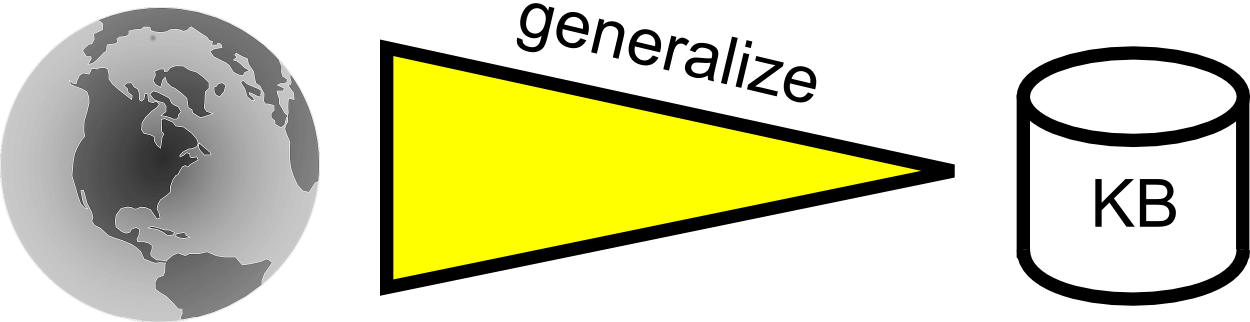
\includegraphics[scale=0.5]{world-model-compression.png}
\end{equation}
The world model is \textit{generated} combinatorially from the set of logic formulas, vaguely reminiscent of a ``basis'' in vector space.  The generative process in logic is much more complicated, contributing to its high \textit{compressive} ability on the one hand, and the \textit{complexity} of learning such formulas on the other hand.

\section{Bottom-up vs top-down representations}

In LBAI the knowledge representation structure is built (\textit{fixed}) from the bottom up (For example, predicate symbols and constant symbols build up propositions, and sets of propositions form theories):
%\begin{equation}
%\mbox{words } \triangleright \mbox{ sentences } \triangleright \mbox{ logical form } \triangleright \mbox{ logical KB}
%\end{equation}
%Thus the structure of the KB is \textit{fixed} by the human designer. % This rigidity is perhaps why learning in logic-based systems is slow.

% In natural language, an idea can be expressed as a concatenation of words, for example:\\
% And it is just a short jump from word concatenations to symbolic logic.  But this jump may land us into a logic-based ``tar pit'', in which everything is theoretically possible, but often too slow in practice.

%It is just a short jump from the expression of ideas as word concatenations to logical form as linear (or tree-like, or graph-like) compositions of symbols:
\begin{equation}
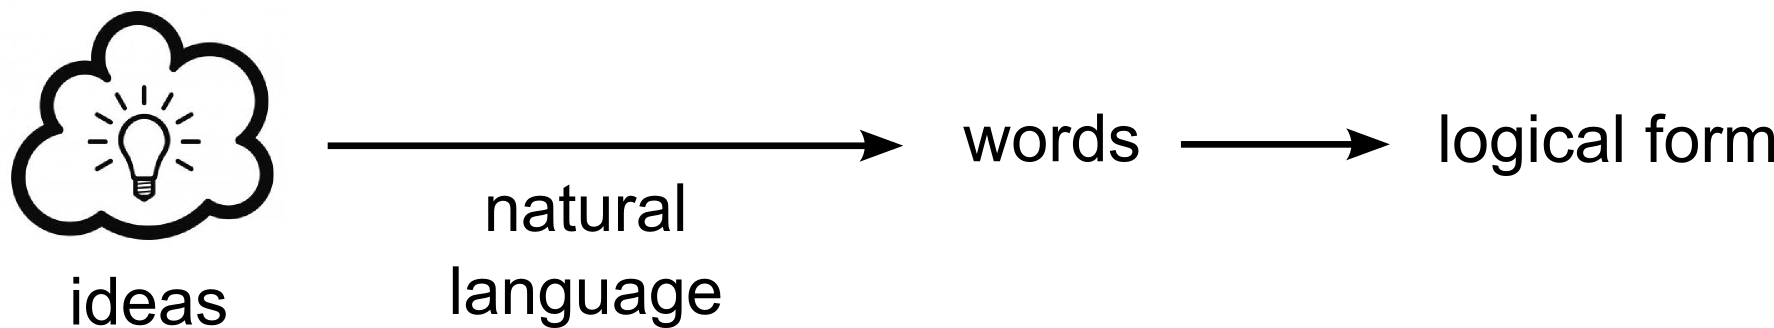
\includegraphics[scale=0.5]{ideas-vs-logical-form.png}
\end{equation}
but is it valid (or profitable) to assume that our mental representations are \textit{isomorphic} to such logical structures?  Or drastically different?

The most serious disadvantage of bottom-up representations lies in the difference between \emp{syntactic distance} and \emp{semantic distance}.  Suppose propositions are built up from an ``alphabet'' of atomic concepts, through the use of a multiplication operation such as tensor product.  We embed atomic concepts into a vector space, in the manner of the Word2Vec algorithm.  Then, using the tensor product, propositions (ie sentences) will be mapped to positions in the tensor-product vector space.  Thus we can measure the \textbf{distance} between any two propositions.  However, this is a \textbf{syntactic} distance.  For example, \textit{``Don't judge a book by its cover''} and \textit{``Clothes do not make the man''} are superficially very different (syntactically distant) but are semantically close.  In a good learning system we need to \textbf{generalize} according to semantic distance.  The embedding of bottom-up representations usually gives us a discrete space with fractal structure, and the metric defined on such a space is always syntactic.

Humans are good at designing symbolic structures, but we don't know how to design \textit{neural} representations which are more or less opaque to us.
Perhaps we could use a neural network acting recurrently on the state vector to \emp{induce} an internal representation of mental space.  ``\textit{Induced by what},'' you ask?  By the very structure of the neural network itself.  In other words, forcing a neural network to \textit{approximate} the ideal operator $R^*$.

From an abstract point of view, we require:
\begin{itemize}
\item $R$ be an endomorphism: $X \rightarrow X$
\item $R$ has a learning algorithm: $R \stackrel{A}{\longmapsto} R^*$
\end{itemize}

$R$ would contain all the knowledge of the KB, so we expect it to be ``large'' (eg. having a huge number of parameters).  We also desire $R$ to possess a \emp{hierarchical} structure because hierarchies are computationally very efficient.  A multi-layer perceptron (MLP) seems to be a good candidate, as it is just a bunch of numbers (weight matrices $W$) interleaved by non-linear activation functions:
\begin{equation}
R(\vect{x}) = \sigmoid(W_1 \sigmoid(W_2 ... \sigmoid(W_L \vect{x} )))
\end{equation}
where $L$ is the number of layers.  MLPs would be our starting point to explore more design options.

In 1991 Siegelmann and Sontag \cite{Siegelmann1991} proved that recurrent neural networks (RNNs) can emulate any Turing machine.  In 1993 James Lo \cite{Lo1993} proved that RNNs can universally approximate any non-linear dynamical system.

The idea of $R$ as an operator acting on the state is inspired by the ``consequence operator'' in logic, usually denoted as $\mbox{Cn}$:
\begin{equation}
\mbox{Cn}(\Gamma) = \{ \mbox{ set of propositions that entails from } \Gamma \; \}
\end{equation}
but the function of $R$ can be broader than logical entailment.  We could use $R$ to perform the following functions which are central to LBAI:
\begin{itemize}
\item \emp{deduction} -- forward- and backward-chaining
\item \emp{abduction} -- finding explanations
\item \emp{inductive learning}
\end{itemize}

Below, we try to formalize the structure of logic from 2 perspectives:
\begin{itemize}
\item Static structure (formulas built from atomic concepts, logic operators, etc)
\item Dynamic structure (mechanisms of proof, inference, etc)
\end{itemize}

\section{Static structure of logic}

\begin{itemize}
\item \emp{truth values} (eg. P(rain tomorrow) = 0.7)
\item \emp{propositional structure} (eg. conjunction: $A \wedge B$) 
\item \emp{sub-propositional structure} (eg. predication: loves(john, mary) )
\item \emp{subsumption structure} (eg. $\mbox{dog} \subseteq \mbox{animal}$)
\end{itemize}

These structures can be ``transplanted'' to the vector space $X$ via:
\begin{itemize}
\item \emp{truth values: } an extra dimension conveying the ``strength'' of states
\item \emp{propositional structure: } eg. conjunction as vector addition,
\begin{equation}
A \wedge B \quad \Leftrightarrow \quad \vect{x}_A + \vect{x}_B + ...
\end{equation}
but we may have to avoid linear dependencies (``clashing'') such as:
\begin{equation}
\vect{x}_3 = a_1 \vect{x}_1 + a_2 \vect{x}_2
\end{equation}
This would force the vector space dimension to become very high.
\item \emp{sub-propositional structure: } eg. tensor products as composition of concept atoms:
\begin{equation}
\mbox{loves(john, pete)} \quad \Leftrightarrow \quad \overrightarrow{john} \otimes \overrightarrow{love} \otimes \overrightarrow{pete}
\end{equation}
\item \emp{subsumption structure: } eg. define the \textbf{positive cone} $C$ such that
\begin{equation}
\mbox{animal} \supseteq \mbox{dog} \quad \Leftrightarrow \quad \overrightarrow{animal} - \overrightarrow{dog} \in C
\end{equation}
\end{itemize}

But the more logical structure we add to $X$, the more it will resemble logic, and this whole exercise becomes pointless.  Remember our original goal is to try something different from logic, by \textit{relaxing} what defines a logical structure.  So we would selectively add features to $X$.

\section{Dynamic structure of logic}

{\color{green}@Andrew: This is where I want to formalize a ``logical system''.  Particularly, the state $X$ has internal structure that I have ignored so far:  $X$ should be a \textbf{set} of propositions.  During deduction, we need to \textbf{select} a few propositions from $X$ and try to \textbf{match} them with existing logic rules (this is the job of the famous \textbf{unifcation} algorithm in logical AI systems).  The selection is part of the control variable $u$ (see below).  We need to decompose the vector $X$ into some analogue of ``propositions'', but I don't know how to do it yet.  Perhaps elucidating the algebraic form of the logic system will help us design the ``vectorization'' scheme.
}

The 2 ``pillar'' algorithms for deduction in LBAI are:

\begin{itemize}
\item \emp{Resolution}:  deducing new propositions (conclusions) from existing ones (premises) \\
\begin{equation}
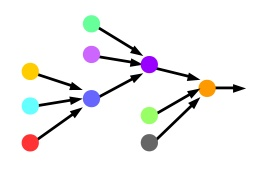
\includegraphics[scale=0.5]{resolution-cartoon.jpg}
\end{equation}
\item \emp{Unificaiton}:  matching a proposition with variables (``holes'') with grounded (``without holes'') propositions \\
\begin{equation}

\includegraphics[scale=0.5]{unification-cartoon.jpg}
\end{equation}
\end{itemize}

The algebraization of first-order predicate logic (a logic whose propositions can have internal variables) is a difficult subject, potentially involving Tarski's cylindrical algebra which the author is unfamiliar with.

Here we introduce a crucial idea: using an \textbf{external memory} to manage the problem of \textbf{variable binding}.  Recall that a \textbf{Turing machine} is just a finite state machine equipped with a \textbf{memory tape};  It could be said that the memory tape is what enables the machine to have Turing-complete computing power.  Similarly, allowing a \textbf{propositional logic} to use an external memory storage for intermediate results, enables it to have the same expressive power as \textbf{predicate logic}.

Below are 2 cartoons illustrating how \textbf{resolution} and \textbf{unification} are performed with the aid of \textbf{external memory}:

{\color{green}@Andrew: I want to formalize these operations.  It may be more important than formalizing the \textbf{static} properties of logic.}

\begin{equation}
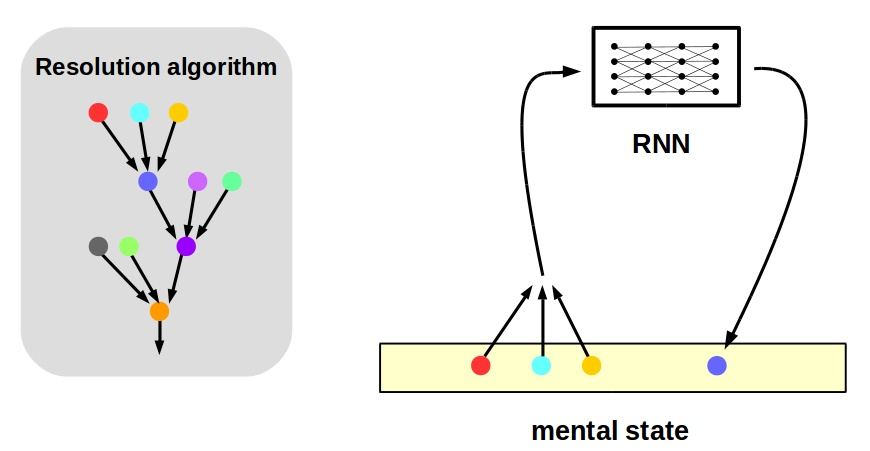
\includegraphics[scale=0.3]{resolution-cartoon-2.jpg}
\end{equation}

\begin{equation}
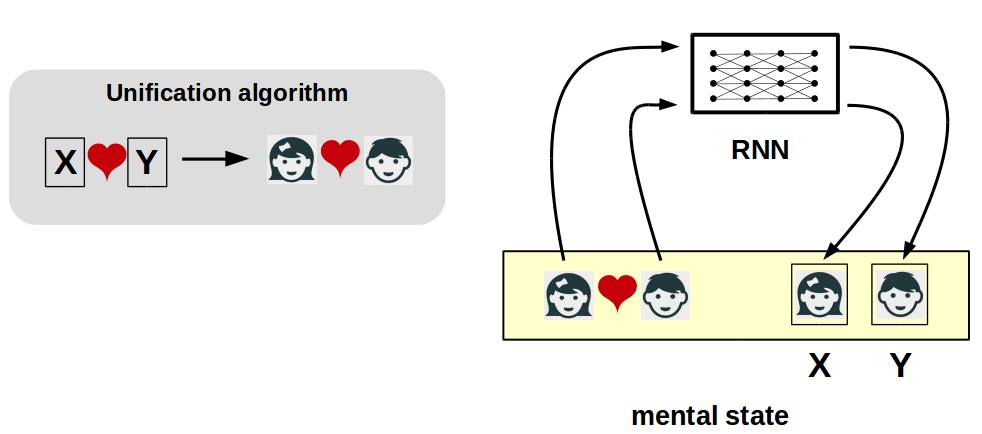
\includegraphics[scale=0.3]{unification-cartoon-2.jpg}
\end{equation}

%%%%%%%%%%%%%%%%%%%%%%%%%%%%%%% Example 1 %%%%%%%%%%%%%%%%%%%%%%%%%%%%%%%
\begin{tcolorbox}[width=\textwidth,colback={white},title={\centering \emp{Example 1: } primary-school arithmetic},colbacktitle=white,coltitle=black]

A recurrent neural network is a \textit{much more powerful} learning machine than a feed-forward network, even if they look the same superficially.

\begin{wrapfigure}{l}{2cm}
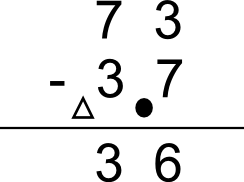
\includegraphics[scale=0.6]{elementary-arithmetic.png}
\end{wrapfigure} 

As an example, consider the way we perform 2-digit subtraction in primary school.  This is done in two steps, and we put a dot on paper to mark ``carry-over''.

The use of the paper is analogous to the ``tape'' in a Turing machine -- the ability to use short-term memory allows us to perform much more complex mental tasks.

We did a simple experiment to train a neural network to perform primary-school subtraction.  The operator is learned easily if we train the two steps \textit{separately}.  The challenge is to find an algorithm that can learn \emp{multi-step} operations by itself.

\end{tcolorbox}
%%%%%%%%%%%%%%%%%%%%%%%%%%%%%%%%%%%%%%%%%%%%%%%%%%%%%%%%%%%%%%%%%%%%%%%%%%

%%%%%%%%%%%%%%%%%%%%%%%%%%%%%%%% Example 2 %%%%%%%%%%%%%%%%%%%%%%%%%%%%%%%
\begin{tcolorbox}[width=\textwidth,colback={white},title={\centering \emp{Example 2: } variable binding in predicate logic},colbacktitle=white,coltitle=black]

The following formula in predicate logic defines the ``grandfather'' relation:

\begin{equation}
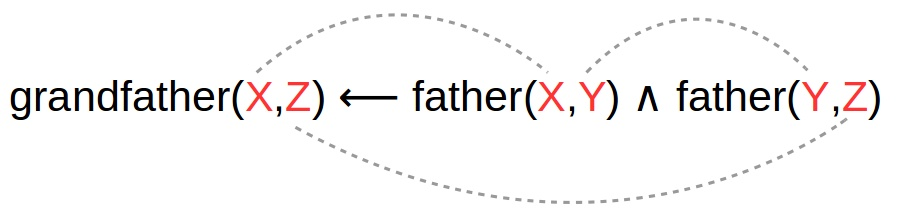
\includegraphics[scale=0.25]{linkage-in-logic-variables.jpg}
\end{equation}

We did a simple experiment to train a neural network to perform primary-school subtraction.  The operator is learned easily if we train the two steps \textit{separately}.  The challenge is to find an algorithm that can learn \emp{multi-step} operations by itself.

\end{tcolorbox}  
%%%%%%%%%%%%%%%%%%%%%%%%%%%%%%%%%%%%%%%%%%%%%%%%%%%%%%%%%%%%%%%%%%%%%%%%%%

\bibliographystyle{plain} % or number or aaai ...
\bibliography{AGI-book}

\end{document}
